\documentclass[11pt,a4paper]{article}
\usepackage[utf8]{inputenc}
\usepackage[english]{babel}
\usepackage{geometry}
\usepackage{graphicx}
\usepackage{amsmath}
\usepackage{amsfonts}
\usepackage{amssymb}
\usepackage{listings}
\usepackage{xcolor}
\usepackage{tikz}
\usepackage{hyperref}
\usepackage{fancyhdr}
\usepackage{enumitem}
\usepackage{booktabs}
\usepackage{microtype}

\usetikzlibrary{shapes,arrows,positioning,fit,backgrounds}

\geometry{margin=1in}
\sloppy
\tolerance=1000
\hbadness=10000
\hypersetup{
    colorlinks=true,
    linkcolor=blue,
    filecolor=magenta,      
    urlcolor=cyan,
    pdftitle={MultiVM Architecture Specification},
    pdfpagemode=FullScreen,
}

\lstset{
    backgroundcolor=\color{gray!10},
    basicstyle=\ttfamily\small,
    keywordstyle=\color{blue},
    commentstyle=\color{green!60!black},
    stringstyle=\color{red},
    breaklines=true,
    frame=single,
    captionpos=b
}

\setlength{\headheight}{14pt}
\pagestyle{fancy}
\fancyhf{}
\rhead{MultiVM Architecture Specification}
\lhead{Version 1.0}
\cfoot{\thepage}

\title{\textbf{MultiVM Architecture Specification} \\ 
       \large{Detailed Structure Documentation for SVM and EVM Integration}}
\author{MultiVM Development Team}
\date{\today}

\begin{document}

\maketitle

\tableofcontents
\newpage

\section{Project Overview}

\subsection{Objective}
The goal is to implement a blockchain that supports both Solana Virtual Machine (SVM) and Ethereum Virtual Machine (EVM). Due to the enormous workload of implementing a chain that supports both SVM and EVM from scratch, our approach is to directly use Solana nodes and Reth nodes as the execution layer and persistence layer for SVM and EVM respectively.

\subsection{Architecture Overview}
The architecture involves several layers: P2P layer, Consensus layer, Account Mapping layer, MultiVM Execution layer, SVM+EVM Execution layer, and Persistence layer.

\textbf{Layer Implementation Distribution:}
\begin{itemize}
    \item \textbf{P2P Layer, Consensus Layer, Account Mapping Layer, and MultiVM Execution Layer}: Implemented by the MultiVM project
    \item \textbf{SVM+EVM Execution Layer}: Provided by Solana nodes and Reth nodes
    \item \textbf{Persistence Layer}: Shared by MultiVM, Solana nodes, and Reth nodes
\end{itemize}

\begin{figure}[h]
\centering
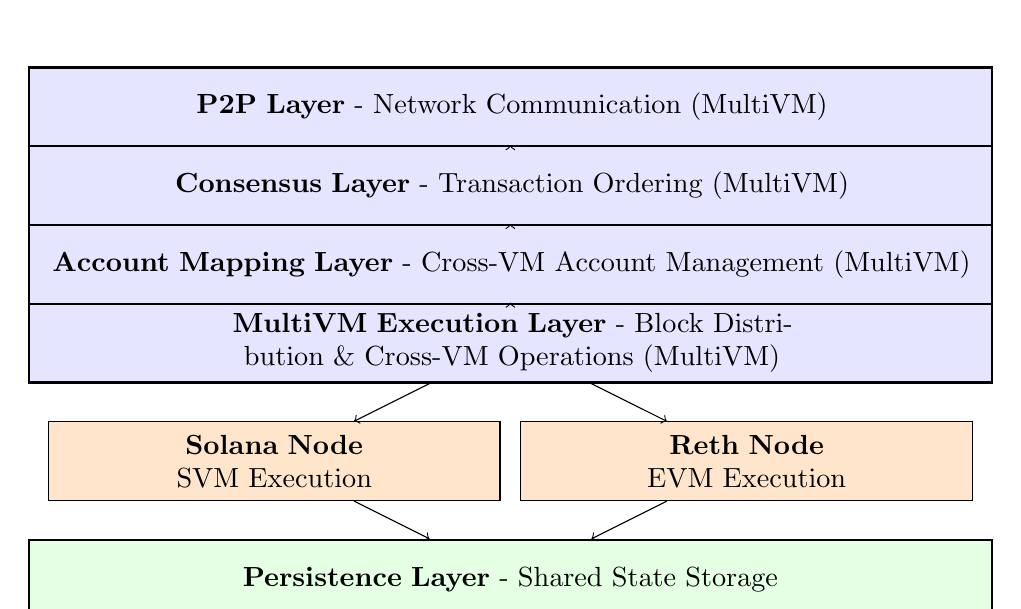
\begin{tikzpicture}[
    layer/.style={rectangle, draw=black, fill=blue!10, text width=12cm, text centered, minimum height=1cm, thick},
    vm/.style={rectangle, draw=black, fill=orange!20, text width=5.5cm, text centered, minimum height=1cm},
    shared/.style={rectangle, draw=black, fill=green!10, text width=12cm, text centered, minimum height=1cm, thick}
]

% Layers implemented by MultiVM
\node[layer] (p2p) at (0, 5) {\textbf{P2P Layer} - Network Communication (MultiVM)};
\node[layer] (consensus) at (0, 4) {\textbf{Consensus Layer} - Transaction Ordering (MultiVM)};
\node[layer] (mapping) at (0, 3) {\textbf{Account Mapping Layer} - Cross-VM Account Management (MultiVM)};
\node[layer] (multivm) at (0, 2) {\textbf{MultiVM Execution Layer} - Block Distribution \& Cross-VM Operations (MultiVM)};

% VM Layer
\node[vm] (solana) at (-3, 0.5) {\textbf{Solana Node} \\ SVM Execution};
\node[vm] (reth) at (3, 0.5) {\textbf{Reth Node} \\ EVM Execution};

% Shared layer
\node[shared] (persistence) at (0, -1) {\textbf{Persistence Layer} - Shared State Storage};

% Arrows
\draw[->] (p2p) -- (consensus);
\draw[->] (consensus) -- (mapping);
\draw[->] (mapping) -- (multivm);
\draw[->] (multivm) -- (solana);
\draw[->] (multivm) -- (reth);
\draw[->] (solana) -- (persistence);
\draw[->] (reth) -- (persistence);

\end{tikzpicture}
\caption{MultiVM Architecture Layer Structure}
\label{fig:architecture}
\end{figure}

\subsection{Design Principles}
The MultiVM architecture follows several key design principles:

\begin{itemize}
    \item \textbf{Reuse of Existing Solutions}: Leverage proven Solana and Reth implementations rather than building from scratch
    \item \textbf{Network Isolation}: Complete isolation of VM nodes from external networks for security and control
    \item \textbf{Unified Consensus}: Single consensus mechanism handling both SVM and EVM transactions
    \item \textbf{Cross-VM Account Management}: Seamless account mapping between different virtual machine environ\-ments
    \item \textbf{Modular Design}: Clear separation of responsibilities across architectural layers
\end{itemize}

\section{Layer Specifications}

\subsection{P2P Layer}
When running Solana and Reth, we disable their P2P networks and Reth networks, retaining the RPC modules but having MultiVM relay and distribute communications.

\textbf{Key Characteristics:}
\begin{itemize}
    \item Solana and Reth nodes are completely unable to communicate with the outside world
    \item P2P module is handled by MultiVM
    \item SVM transactions, EVM transactions, and consensus information sent by users are completely forwarded and broadcast by the MultiVM module
    \item Information validation work is handled by the SVM and EVM execution layers
\end{itemize}

\textbf{Communication Flow:}
\begin{enumerate}
    \item External users and DApps send transactions to MultiVM P2P layer
    \item MultiVM P2P layer receives and validates transaction format
    \item MultiVM forwards transactions to consensus layer for ordering
    \item After consensus, transactions are distributed to appropriate execution layers
    \item Responses are relayed back through MultiVM to external clients
\end{enumerate}

\textbf{Network Configuration:}
\begin{itemize}
    \item \textbf{Solana Node}: All P2P ports disabled, no external peer connections
    \item \textbf{Reth Node}: Discovery disabled, no peer-to-peer networking
    \item \textbf{MultiVM}: Acts as sole network interface for the entire system
\end{itemize}

\subsection{Consensus Layer}
The consensus will be completely independent of the SVM and EVM execution layers. This process will simultaneously handle both SVM transactions and EVM transactions.

\textbf{Functions:}
\begin{itemize}
    \item Independent consensus mechanism
    \item Simultaneous processing of SVM and EVM transactions
    \item Unified transaction ordering
    \item Cross-VM transaction coordination
\end{itemize}

\textbf{Consensus Process:}
\begin{enumerate}
    \item Receive mixed transaction batches from P2P layer
    \item Apply consensus algorithm to determine global transaction ordering
    \item Separate transactions by target VM (SVM/EVM/Special)
    \item Generate unified blocks containing both SVM and EVM components
    \item Coordinate execution across both virtual machines
    \item Ensure atomic commitment of block state
\end{enumerate}

\textbf{Transaction Ordering:}
The consensus layer maintains a unified ordering of all transactions regardless of their target virtual machine, ensuring consistent global state across the entire system.

\subsection{Account Mapping Layer}
This layer detects special account binding transactions, handles user account binding, and calls SVM and EVM execution layers to check whether transaction addresses have corresponding MultiVM accounts.

\textbf{Responsibilities:}
\begin{itemize}
    \item Detection of special account binding transactions
    \item Processing of user account binding operations
    \item Verification of MultiVM account existence across execution layers
    \item Maintenance of cross-VM account relationship database
    \item Account state synchronization between VMs
\end{itemize}

\textbf{Account Binding Workflow:}
\begin{enumerate}
    \item Detect incoming special binding transactions
    \item Validate account ownership proofs
    \item Check existing account mappings
    \item Create or update account binding relation\-ships
    \item Update account mapping database
    \item Notify relevant execution layers of binding changes
\end{enumerate}

\textbf{Account Lookup Process:}
\begin{itemize}
    \item Query MultiVM account database for existing mappings
    \item Cross-reference with SVM and EVM execution layers
    \item Validate account states across virtual machines
    \item Return unified account information to requesting layer
\end{itemize}

\subsection{MultiVM Execution Layer}
Used to handle all unified operations, such as block parsing and distribution, future cross-VM execution, and SVM and EVM state exchange.

\textbf{Core Functions:}
\begin{itemize}
    \item Block parsing and distribution
    \item Cross-VM execution coordination
    \item SVM and EVM state exchange
    \item Unified operation management
    \item Transaction routing to appropriate execution layers
\end{itemize}

\textbf{Block Processing Workflow:}
\begin{enumerate}
    \item Receive unified blocks from consensus layer
    \item Parse blocks into SVM and EVM components
    \item Route SVM transactions to Solana execution engine
    \item Route EVM transactions to Reth execution engine
    \item Process special MultiVM transactions internally
    \item Coordinate state updates across virtual machines
    \item Aggregate execution results and update persistence layer
\end{enumerate}

\textbf{Cross-VM Coordination:}
\begin{itemize}
    \item Manage state consistency between SVM and EVM environments
    \item Handle cross-VM account operations
    \item Coordinate atomic transactions affecting multiple VMs
    \item Maintain unified view of system state
\end{itemize}

\subsection{SVM+EVM Execution Layer}
Executes specific SVM and EVM transactions and updates account states.

\textbf{Components:}
\begin{itemize}
    \item \textbf{Solana Node}: Handles SVM transaction execution with complete runtime environment
    \item \textbf{Reth Node}: Handles EVM transaction execution with full smart contract support
    \item Both nodes operate with disabled networking capabilities
    \item Communication only through MultiVM-controlled RPC inter\-faces
\end{itemize}

\textbf{Solana Node Configuration:}
\begin{itemize}
    \item Standard Solana validator with networking disabled
    \item JSON-RPC interface enabled for MultiVM communication
    \item All P2P functionality completely disabled
    \item Consensus mechanisms bypassed
\end{itemize}

\textbf{Reth Node Configuration:}
\begin{itemize}
    \item Standard Reth node with P2P disabled
    \item Engine API enabled for block submission
    \item Discovery and peer networking disabled
    \item Development mode for external block control
\end{itemize}

\textbf{Execution Process:}
\begin{enumerate}
    \item Receive transaction batches from MultiVM Execution Layer
    \item Execute transactions within respective virtual machine environments
    \item Update local account states and storage
    \item Generate execution receipts and state changes
    \item Report results back to MultiVM Execution Layer
    \item Commit state changes to persistence layer
\end{enumerate}

\subsection{Persistence Layer}
Saves EVM and SVM states, stores SVM and EVM account mappings, etc.

\textbf{Storage Contents:}
\begin{itemize}
    \item EVM state data (accounts, contracts, storage)
    \item SVM state data (accounts, programs, data)
    \item Account mapping relationships between VMs
    \item Transaction history for both virtual machines
    \item Cross-VM operation logs
    \item System configuration and metadata
\end{itemize}

\textbf{Data Management:}
\begin{itemize}
    \item Shared storage accessible by all system components
    \item Atomic updates across virtual machine boundaries
    \item Consistent snapshots of system state
    \item Efficient querying of cross-VM account relationships
\end{itemize}

\textbf{Storage Architecture:}
\begin{enumerate}
    \item \textbf{VM-Specific Storage}: Native storage formats for Solana and Reth
    \item \textbf{Mapping Database}: Cross-VM account relationship storage
    \item \textbf{Unified Metadata}: System-wide configuration and state information
    \item \textbf{Transaction Logs}: Complete audit trail of all operations
\end{enumerate}

\section{Account Model}

When an account A (A can be an SVM account or EVM account) first appears in our system, the system automatically creates a MultiVM account M and binds M and A together. Subsequently, users can perform operations to bind the corresponding other platform account B with M, thus achieving account association between SVM and EVM platforms, while also having M for convenient management.

\begin{figure}[h]
\centering
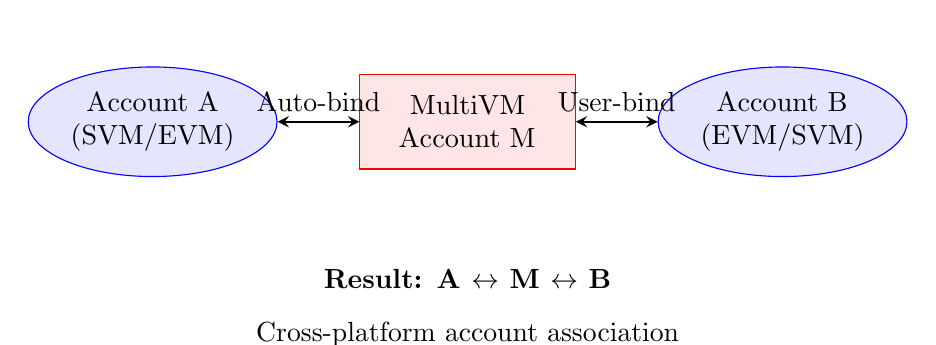
\begin{tikzpicture}[
    account/.style={ellipse, draw=blue, fill=blue!10, text width=2cm, text centered, minimum height=1cm},
    multivm/.style={rectangle, draw=red, fill=red!10, text width=2.5cm, text centered, minimum height=1.2cm},
    arrow/.style={thick, <->, >=stealth}
]

% Initial state
\node[account] (accountA) at (-4, 3) {Account A \\ (SVM/EVM)};
\node[multivm] (multivmM) at (0, 3) {MultiVM \\ Account M};
\node[account] (accountB) at (4, 3) {Account B \\ (EVM/SVM)};

% Relationships
\draw[arrow] (accountA) -- (multivmM) node[midway, above] {Auto-bind};
\draw[arrow] (multivmM) -- (accountB) node[midway, above] {User-bind};

% Final relationship
\node at (0, 1) {\textbf{Result: A $\leftrightarrow$ M $\leftrightarrow$ B}};
\node at (0, 0.3) {Cross-platform account association};

\end{tikzpicture}
\caption{Account Binding Model}
\label{fig:account-model}
\end{figure}

\textbf{Binding Process:}
\begin{enumerate}
    \item System automatically creates MultiVM account M when account A first appears
    \item Automatic binding: A $\leftrightarrow$ M
    \item User can bind additional account B: B $\leftrightarrow$ M
    \item Final relationship: A $\leftrightarrow$ M $\leftrightarrow$ B
\end{enumerate}

\textbf{Binding Transaction Processing:}
The binding process allows users to send special type transactions, which are processed by the MultiVM execution layer and do not go through the SVM+EVM execution layer.

\subsection{Account Types}
\begin{itemize}
    \item \textbf{SVM Accounts}: Native Solana accounts with Ed25519 public keys
    \item \textbf{EVM Accounts}: Ethereum-compatible accounts with secp256k1 public keys
    \item \textbf{MultiVM Accounts}: System-generated accounts that serve as binding anchors
\end{itemize}

\subsection{Account Binding Operations}
\begin{enumerate}
    \item \textbf{Initial Account Creation}: When account A first interacts with the system
    \begin{itemize}
        \item System detects new account A
        \item Automatically generates MultiVM account M
        \item Creates binding A $\leftrightarrow$ M
        \item Records binding in account mapping database
    \end{itemize}
    
    \item \textbf{Cross-Platform Binding}: User-initiated binding of second account
    \begin{itemize}
        \item User submits special binding transaction
        \item System validates ownership of both accounts
        \item Creates binding B $\leftrightarrow$ M
        \item Updates account mapping database
        \item Establishes complete relation\-ship A $\leftrightarrow$ M $\leftrightarrow$ B
    \end{itemize}
\end{enumerate}

\subsection{Account Management Features}
\begin{itemize}
    \item \textbf{Unified Balance Tracking}: View combined balances across bound accounts
    \item \textbf{Cross-VM Transfers}: Transfer assets between bound SVM and EVM accounts
    \item \textbf{Permission Management}: Set permissions for cross-VM operations
    \item \textbf{Binding History}: Complete audit trail of account binding operations
\end{itemize}

\section{Transaction Model}

We will be able to process three types of transactions:

\subsection{EVM Transactions}
Standard Ethereum-compatible transactions that are processed by the Reth node in the SVM+EVM execution layer.

\textbf{Transaction Structure:}
\begin{itemize}
    \item Standard Ethereum transaction format
    \item Full compatibility with existing Ethereum tooling
    \item Gas-based fee model
    \item Smart contract interaction support
\end{itemize}

\textbf{Processing Flow:}
\begin{enumerate}
    \item Transaction received by P2P layer
    \item Validated and ordered by consensus layer
    \item Routed to Reth node by MultiVM execution layer
    \item Executed within EVM environment
    \item State changes committed to persistence layer
\end{enumerate}

\subsection{SVM Transactions}
Standard Solana-compatible transactions that are processed by the Solana node in the SVM+EVM execution layer.

\textbf{Transaction Structure:}
\begin{itemize}
    \item Standard Solana transaction format
    \item Instruction-based execution model
    \item Fixed fee structure
    \item Program interaction support
\end{itemize}

\textbf{Processing Flow:}
\begin{enumerate}
    \item Transaction received by P2P layer
    \item Validated and ordered by consensus layer
    \item Routed to Solana node by MultiVM execution layer
    \item Executed within SVM environment
    \item State changes committed to persistence layer
\end{enumerate}

\subsection{Special Type Transactions}
Custom transactions for MultiVM-specific operations such as account binding, processed exclusively by the MultiVM execution layer without involving the SVM+EVM execution layer.

\textbf{Transaction Types:}
\begin{itemize}
    \item \textbf{Account Binding}: Link accounts across virtual machines
    \item \textbf{Cross-VM Transfers}: Move assets between bound accounts
    \item \textbf{System Configuration}: Update MultiVM system parameters
    \item \textbf{Account Management}: Modify account permissions and settings
\end{itemize}

\textbf{Processing Flow:}
\begin{enumerate}
    \item Transaction received by P2P layer
    \item Validated and ordered by consensus layer
    \item Processed directly by MultiVM execution layer
    \item Account mapping layer updated as needed
    \item Changes committed to persistence layer
\end{enumerate}

\begin{figure}[h]
\centering
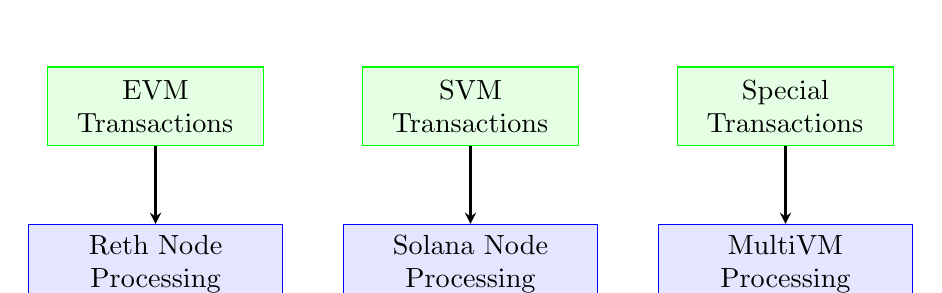
\begin{tikzpicture}[
    tx/.style={rectangle, draw=green, fill=green!10, text width=2.5cm, text centered, minimum height=1cm},
    processing/.style={rectangle, draw=blue, fill=blue!10, text width=3cm, text centered, minimum height=1cm},
    arrow/.style={thick, ->, >=stealth}
]

% Transaction types
\node[tx] (evm_tx) at (-4, 4) {EVM \\ Transactions};
\node[tx] (svm_tx) at (0, 4) {SVM \\ Transactions};
\node[tx] (special_tx) at (4, 4) {Special \\ Transactions};

% Processing destinations
\node[processing] (reth_proc) at (-4, 2) {Reth Node \\ Processing};
\node[processing] (solana_proc) at (0, 2) {Solana Node \\ Processing};
\node[processing] (multivm_proc) at (4, 2) {MultiVM \\ Processing};

% Arrows
\draw[arrow] (evm_tx) -- (reth_proc);
\draw[arrow] (svm_tx) -- (solana_proc);
\draw[arrow] (special_tx) -- (multivm_proc);

\end{tikzpicture}
\caption{Transaction Processing Model}
\label{fig:transaction-model}
\end{figure}

\subsection{Transaction Lifecycle}
\begin{enumerate}
    \item \textbf{Submission}: Transaction submitted to MultiVM P2P layer
    \item \textbf{Validation}: Basic format and signature validation
    \item \textbf{Classification}: Determine transaction type (EVM/SVM/Special)
    \item \textbf{Consensus}: Global ordering through consensus mechanism
    \item \textbf{Routing}: Distribution to appropriate execution layer
    \item \textbf{Execution}: VM-specific or MultiVM processing
    \item \textbf{State Update}: Commit changes to persistence layer
    \item \textbf{Confirmation}: Return execution results to client
\end{enumerate}

\section{Block Model}

For compatibility considerations, our blocks will consist of two parts: one part is a legal SVM block, and the other part is a legal ETH block. They are packaged together through a consensus process.

\begin{align}
Block_{MultiVM} = \{Block_{SVM}, Block_{ETH}\}
\end{align}

Where:
\begin{align}
Block_{SVM} &= \text{Legal Solana block structure} \\
Block_{ETH} &= \text{Legal Ethereum block structure}
\end{align}

\textbf{Block Composition:}
\begin{itemize}
    \item \textbf{SVM Block Component}: Contains SVM transactions and follows Solana block format
    \item \textbf{ETH Block Component}: Contains EVM transactions and follows Ethereum block format
    \item \textbf{Unified Consensus}: Both components are packaged together through a single consensus process
\end{itemize}

\begin{figure}[h]
\centering
\begin{tikzpicture}[
    block/.style={rectangle, draw=black, fill=yellow!20, text width=4cm, text centered, minimum height=2cm, thick},
    unified/.style={rectangle, draw=red, fill=red!10, text width=10cm, text centered, minimum height=3cm, thick}
]

\node[unified] (unified_block) at (0, 0) {};
\node[block] (svm_block) at (-2.5, 0) {\textbf{SVM Block} \\ \textbullet\, SVM Transactions \\ \textbullet\, Solana Format \\ \textbullet\, Rewards \\ \textbullet\, Block Time};
\node[block] (eth_block) at (2.5, 0) {\textbf{ETH Block} \\ \textbullet\, EVM Transactions \\ \textbullet\, Ethereum Format \\ \textbullet\, Receipts \\ \textbullet\, Gas Usage};

\node at (0, -2) {\textbf{MultiVM Unified Block}};
\node at (0, -2.5) {Single Consensus Process};

\end{tikzpicture}
\caption{Block Structure Model}
\label{fig:block-model}
\end{figure}

\subsection{Block Generation Process}
\begin{enumerate}
    \item \textbf{Transaction Collection}: Gather pending transactions from all sources
    \item \textbf{Transaction Separation}: Sort transactions by target VM
    \item \textbf{Consensus Application}: Apply unified consensus to determine block contents
    \item \textbf{Block Construction}: Create valid SVM and ETH block structures
    \item \textbf{Cross-VM Validation}: Ensure consistency across block components
    \item \textbf{Block Finalization}: Package into unified MultiVM block
    \item \textbf{Distribution}: Send to execution layers for processing
\end{enumerate}

\subsection{Block Structure Details}
\textbf{SVM Block Component:}
\begin{itemize}
    \item Standard Solana block header with MultiVM modifications
    \item SVM transactions in native Solana format
    \item Reward distribution information
    \item Block timing and slot information
\end{itemize}

\textbf{ETH Block Component:}
\begin{itemize}
    \item Standard Ethereum block header with MultiVM modifications
    \item EVM transactions in native Ethereum format
    \item Transaction receipts and event logs
    \item Gas usage and fee information
\end{itemize}

\textbf{MultiVM Metadata:}
\begin{itemize}
    \item Cross-VM transaction references
    \item Account binding updates
    \item Consensus proof information
    \item System state checksums
\end{itemize}

\section{Implementation Architecture}

\subsection{Process Configuration}

\textbf{Solana Node Configuration:}
\begin{itemize}
    \item P2P network completely disabled
    \item RPC module retained for MultiVM communication
    \item Network isolation from external environment
    \item Consensus mechanisms bypassed
\end{itemize}

\textbf{Reth Node Configuration:}
\begin{itemize}
    \item P2P network completely disabled
    \item RPC module retained for MultiVM communication
    \item Network isolation from external environment
    \item Mining and block production disabled
\end{itemize}

\textbf{MultiVM Core:}
\begin{itemize}
    \item Handles all external network communication
    \item Relays and distributes transactions to appropriate execution layers
    \item Manages consensus process
    \item Coordinates cross-VM operations
\end{itemize}

\subsection{Communication Protocols}

\textbf{MultiVM to Solana Communication:}
\begin{itemize}
    \item JSON-RPC interface for transaction submission
    \item Custom APIs for block notification
    \item State query interfaces
    \item Configuration update mechanisms
\end{itemize}

\textbf{MultiVM to Reth Communication:}
\begin{itemize}
    \item Engine API for block submission
    \item JSON-RPC for transaction processing
    \item State synchronization interfaces
    \item Administrative control APIs
\end{itemize}

\subsection{Communication Flow}

\begin{figure}[h]
\centering
\begin{tikzpicture}[
    external/.style={rectangle, draw=green, fill=green!10, text width=2cm, text centered, minimum height=1cm},
    multivm/.style={rectangle, draw=blue, fill=blue!10, text width=3cm, text centered, minimum height=1.5cm},
    node/.style={rectangle, draw=orange, fill=orange!10, text width=2.5cm, text centered, minimum height=1cm},
    arrow/.style={thick, ->, >=stealth}
]

% External sources
\node[external] (users) at (0, 6) {Users \\ \& DApps};

% MultiVM layer
\node[multivm] (multivm_core) at (0, 4) {\textbf{MultiVM Core} \\ \textbullet\, P2P Handling \\ \textbullet\, Consensus \\ \textbullet\, Distribution};

% Node layer
\node[node] (solana_node) at (-3, 2) {Solana Node \\ (Isolated)};
\node[node] (reth_node) at (3, 2) {Reth Node \\ (Isolated)};

% Storage
\node[multivm] (storage) at (0, 0) {\textbf{Shared Storage} \\ Persistence Layer};

% Communication flows
\draw[arrow] (users) -- (multivm_core) node[midway, right] {All External Communication};
\draw[arrow] (multivm_core) -- (solana_node) node[midway, above left] {SVM Txs};
\draw[arrow] (multivm_core) -- (reth_node) node[midway, above right] {EVM Txs};
\draw[arrow] (solana_node) -- (storage);
\draw[arrow] (reth_node) -- (storage);
\draw[arrow] (multivm_core) -- (storage);

% Isolation indicators
\draw[dashed, red] (-4.5, 1.5) rectangle (-1.5, 2.5);
\draw[dashed, red] (1.5, 1.5) rectangle (4.5, 2.5);
\node[red] at (-3, 1) {Network Isolated};
\node[red] at (3, 1) {Network Isolated};

\end{tikzpicture}
\caption{Communication and Isolation Architecture}
\label{fig:communication}
\end{figure}

\subsection{Deployment Configuration}

\textbf{System Requirements:}
\begin{itemize}
    \item Solana validator binary with networking disabled
    \item Reth node binary with P2P disabled
    \item MultiVM core process with full networking capabilities
    \item Shared storage system accessible by all components
\end{itemize}

\textbf{Network Configuration:}
\begin{itemize}
    \item All external traffic routed through MultiVM core
    \item Solana and Reth nodes bound to localhost only
    \item No direct external access to VM execution nodes
    \item RPC interfaces secured and controlled by MultiVM
\end{itemize}

\textbf{Process Management:}
\begin{itemize}
    \item Independent process lifecycle management
    \item Automatic restart and recovery mechanisms
    \item Health monitoring and status reporting
    \item Resource allocation and limits
\end{itemize}

\section{System Integration}

\subsection{Data Flow Architecture}
The complete data flow through the MultiVM system follows a structured pattern:

\begin{enumerate}
    \item \textbf{Transaction Ingestion}: External transactions enter through P2P layer
    \item \textbf{Consensus Processing}: Unified ordering and validation
    \item \textbf{Account Resolution}: Cross-VM account mapping and validation
    \item \textbf{Execution Routing}: Distribution to appropriate virtual machines
    \item \textbf{State Coordination}: Synchronization across execution environments
    \item \textbf{Persistence Management}: Atomic storage of all state changes
\end{enumerate}

\subsection{Cross-VM Operation Coordination}
Special handling for operations that span multiple virtual machines:

\begin{itemize}
    \item \textbf{Account Binding Operations}: Managed entirely by MultiVM layer
    \item \textbf{Cross-VM Asset Transfers}: Coordinated between bound accounts
    \item \textbf{State Synchronization}: Ensuring consistency across VM boundaries
    \item \textbf{Error Handling}: Rollback mechanisms for failed cross-VM operations
\end{itemize}

\subsection{System Monitoring and Management}
\begin{itemize}
    \item Real-time monitoring of all system components
    \item Health checks for Solana and Reth node processes
    \item Performance metrics collection and reporting
    \item Administrative interfaces for system configuration
    \item Logging and audit trail maintenance
\end{itemize}

\section{Conclusion}

The MultiVM architecture provides a practical solution for supporting both SVM and EVM within a single blockchain system by leveraging existing, proven implementations of Solana and Reth nodes while providing the necessary coordination and management layers. The design ensures compatibility with both ecosystems while maintaining clear separation of concerns across the architec\-tural layers.

This approach minimizes development complexity by reusing existing virtual machine implementations while providing the necessary infrastructure for cross-VM account management, transaction processing, and unified consensus.

The modular design allows for independent development and maintenance of each layer while ensuring seamless integration and operation of the complete system. The network isolation approach provides security and control while maintaining full functionality of both virtual machine environments.

\end{document} 